\documentclass{standalone}

\usepackage{circuitikz}

\begin{document}
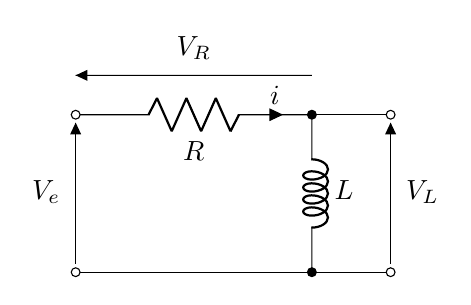
\begin{tikzpicture}
	\draw (0,0) 
	to[R, l_=$R$, o-, i=$i$] (3,0) 
	to[L, l=$L$, *-] (3,-2) 
	to[short,-*](3,-2);

    \draw (3,0) 
    to[short,-o](4,0);
    
	%input
	\draw (0,-0.1)
	to[short, l_=$V_{e}$](0,-1.9) ;
    \draw (0,-2) 
    to[short,o-o](4,-2);

    \draw (3,0.5)
	to[short, l_=$V_{R}$](0,0.5);
    \draw (0,0.5) coordinate[inputarrow,rotate=180];

	\draw (0,-0.1) coordinate[inputarrow,rotate=90];
	% output
	\draw (4,-0.1)
	to[short, l=$V_{L}$](4,-1.9);
	\draw (4,-0.1) coordinate[inputarrow,rotate=90];
\end{tikzpicture}
\end{document}